\documentclass[11pt]{article}
\usepackage[margin=1in]{geometry}
\usepackage{amsfonts, amsmath, amssymb}
\usepackage{mhchem}
\usepackage{parskip}
\usepackage{graphicx}
\graphicspath{.}
\usepackage{subcaption}
\usepackage{placeins}
\usepackage[utf8]{inputenc} 
\usepackage[T1]{fontenc} 
\usepackage{mathpazo} % Palatino font
\usepackage[backend=biber,style=apa]{biblatex}
\addbibresource{{~/Zotero/Zotero.bib}}
\usepackage{fancyhdr}
\usepackage{pdfpages}

\pagestyle{fancy}
\fancyhead{}
\fancyfoot{}
\fancyhead[L]{\MakeUppercase{CHEM3003}}
\fancyhead[R]{\thepage}
\fancyfoot[L]{\textit{Aaron Copeland} | 19765288}
\setlength{\parindent}{0pt}

\begin{document}

\begin{titlepage} 
\newcommand{\HRule}{\rule{\linewidth}{0.5mm}} 
	
	\center % Centre everything on the page

	
	\textsc{\LARGE Curtin University}\\[1.5cm] % Main heading such as the name of your university/college
	
	\textsc{\Large Research, Leadership and Entrepreneurship in Science 2}\\[0.5cm] % Major heading such as course name
	
	\textsc{\large NPSC3000}\\[0.5cm] % Minor heading such as course title
	
	\HRule\\[0.4cm]
	
	{\huge\bfseries Portfolio}\\[0.4cm] % Title of your document
	
	\HRule\\[1.5cm]
	
	\begin{minipage}{0.5\textwidth}
		\begin{flushleft}
			\large
			\textit{Author}\\
			A.D. \textsc{Copeland}\\
                        \textit{ID}: 19765288\\
                        \textit{Email}: \texttt{19765288@student.curtin.edu.au}\\
                        \textit{Due Date}: 29 September 2023
		\end{flushleft}
	\end{minipage}
	~
	\begin{minipage}{0.4\textwidth}
		\begin{flushright}
			\large
			\textit{Unit Coordinator}\\
			Assoc. Prof. Katarina \textsc{Miljkovic}\\ % Supervisor's name
		\end{flushright}
	\end{minipage}
	
	% If you don't want a supervisor, uncomment the two lines below and comment the code above
	%{\large\textit{Author}}\\
	%John \textsc{Smith} % Your name
	
	%------------------------------------------------
	%	Date
	%------------------------------------------------

	\vfill\vfill % Position the date 3/4 down the remaining page

    \raggedright
    
	\large\today % Date, change the \today to a set date if you want to be precise
	
\end{titlepage}

\section{Reflections}

\subsection{Finding a comp chem workflow}
\subsection{Pawsey Tour}

On Thursday March 30th the Curtin Computational Chemistry group, along with three visiting Italian Masters students, toured the Pawsey Supercomputing facility in Technology Park near the Curtin University Campus. The visiting students were being introduced to the prospect of studying a PhD in Australia and shown what Curtin has to offer. I found it valuable chatting with these students. They seemed open to the idea of completing a PhD in Australia, Perth specifically. They liked our mild weather and location. I think the location of study is important in reinforcing positive learning and feeling towards studying. I haven't properly considered studying or working oversear. I'm definitely not opposed to it, but chatting with the students has made me concious that I need to consider the town and surrounds of a possible place I might move to. I have ideas about countries that I would like to study in, but countries are so vast in culture, climate and people that I now know I have to be specific in my search for a host town or city (if or when I choose to look seriously at oversear study!).

The tour started with a presentation about the history and current specifications of the Pawsey supercomputers and the precinct itself. This was a fairly generic presentation, but interesting nonetheless. I was particularly intrigued by the centers used of an underground aquify to aid in watercooling the supercomputers. This is an ingenious way of reducing grid power requirements for the supercomputers. I can tell that a lot of planning went into developing the Pawsey center. After this we got to peer through the windows to where the supercomputers (and a small quantum computer) were housed. Figure~??? shows a photograph of my view. While the supercomputers are much larger than any other computer I've seen in person, they also appeared quite small. A few students on the tour gave a small snicker upon seeing it for the first time. I suppose we were expecting an super-sized computer! I'm somewhat glad at seeing how compact the system was, given its power output (and power requirements). It is an impressive feat of engineering.

After gazing at the black boxes that make my project possible I chatted with one of the Pawesy technicians. I'd read a recent article for a seperate university unit. The article covered the consequences and worries about computer processor manufacturing in Taiwan with the current tension surrounding China trying to gain ownership of the country. With all of the processors that are necessary for the supercomputer, I asked the technician whether Pawsey has any risk mitigation or plans if issues in Taiwan escalated and crippled the worlds primary computer processor manufacturer. The conversation was short, but the technician said that the processor vendors would be directly effected and Pawesy was well equipped with stores of spare parts for the current supercomputer outfit. They mentioned that while it wasn't a current concern for Pawesy, it would be beneficial to add it to the centers discussions. I was pleased to have potentially add a possibly important point to the centers discussions. I am a stakeholder after all! While I wouldn't consider myself politically literate or focussed, I think this reminds me why knowing what is going on around the world is important, even for just using a supercomputer for a university project.

\subsection{Learning a codebase}
\subsection{Super Computer vs. Laptop Computer}

I had to run a computer simulation for my project, but it was actually several simuations that would be run in a sequence. This was going to be orchestrated using a shell script, but a may have misheard my supervisor at some point because I thought they said I had to run this simulation on my laptop, not the supercomputer. I thought I heard that the shell script was written for the Z shell and not Bash and that the supercomputer did not have Z shell, but my personal computer did. I ran the simulation. It took three days to finish with my laptop fans and processor going full tilt. When I saw my supervisor after this, they said that running it on the supercomputer was fine, so we reran the simulation. It finished that same day. This comparison shows me the computing power difference of a laptop and a supercomputer - a lot! I already knew this, but having an unusable laptop for three days wasn't ideal when I still have things I could be doing on it. I have a new found appreciation of being able to connect remotely to a machine to complete a job or simulation and having the perfomance of my host machine be untouched.

\subsection{Making Mistakes}
\subsection{Supervisor being away}
\subsection{Mid-year Presentations}
\subsection{My Understanding of Chemistry}
\subsection{Plain Text talk and TeXMacs}
\subsection{Slumps vs. Pumps}

I have struggled throughout this year with my motivation in my university work and my project. I sometimes find it difficult to find meaning and passion in the work that I should be doing and it feels like a cloud is covering how I really feel (that I do trully enjoy this work!). These struggles also enxtend to my personal activities. Thankfully, I've been inspired by the great bodybuilder Arnold Schwarzenegger to strive for somethink called ``the pump.'' The pump is the feeling of your body being extremely strong and tight when working out and it feels great. This was what I think about when I'm struggling to be active - that I could get the pump - and it's typically the nudge I need to get back into doing physical activity that I like and makes me feel good. So, recently when I've been struggly with my work, I've considered ``the pump'' in terms of working my brain. This has helped me transition out of slumps of being unproductive to getting work done. Hard work of any kind doesn't seem attractive at first glance, so it's easy to brush it off, but just starting with something small makes it easier to continue and try and find the elusive pump.

\subsection{Thinking about Honours}

With my struggles throughout the year, I've had doubts about my abilty and drive to continue on to the honours-year of my degree. Honours is a big commitment and a whole extra year of study. Being so close to having a bachelor's degree and not having a job or money at the moment makes me conscious of my position in society and expecations that I should be a good citizen and get a job as soon as possible and work until death for the greater good of the country - or something like that... I feel better that I've taken more time to think about honours and understand its importance in my academic journey. I still think I would like to be a career researcher and honours is an important stepping stone for this. I understand the challenge of honours and, despite recent struggles, I know I am capable of achieving what I want academically and I do enjoy the fight. I'm fortunate and grateful that I have so many options for next year; do honours, take the intermediate exit award and get a chemist job, take the exit award and get a job in the coffee industry, or something else I haven't considered! I think I have more or less settled on doing honours and feel confident with my choice.

\subsection{Wrinting Units vs. science}

I've chosen to use my elective units this year to complete two writing units. While I could be have used these units to study more chemistry, I thought that extending my writing abilities would be something useful for me as I have struggled with writing generally in different forms. Since I want to pursue a career in academia, journal article writing would be my main publishing form. I already have a decent grasp on this style of writing and understand its value in communicating scientific information to fellow researchers. However, this is a relatively small target audience, and I feel as though scientific information should be accessible to the masses to increase general understanding of the world around us and beyound. Journal articles are not always written in a way that can be well understood by a general audience. This is why I have taken these writing units, to better my skills at writing in creative non-fiction and feature article writing. These styles are more suited to general audiences and can use different techniques to get readers interested in topics they might not usually be. While I may spend most of my career writing in the scientific style required for journal articles, if I want my research to be seen by the masses, I need to know how to show them - and I think the forms I have learnt and practice as part of these units has helped significantly (so much so, that I had considerations of doing a masters degree in writing and pursuing a career through that pathway).

\subsection{Conducting Peer reviews}
\subsection{Being in a new cohort}

Having to redo NPSC3000 this year meant that I was a part of a new cohort of Advanced Science students. Previously, a change like this would have caused me significant anxiety, but I'm happy to say that this wasn't the case. A was already familar with the Advance Science chemistry major students from this cohort, so this eased any tension I had. While I haven't has any ground-breaking chats with my fellow students, they all seem pleasant to be around and engaged with science throught their projects. I feel as though this experience is important for building my adaptability for working with new people as I will have to join a workplace in the future and meet a new team of people (a cohort in a way).

\subsection{Generative AI}

While I don't consider myself a trend-chasing, I do like to keep an understanding in trends, typically in technology. However, with all this talk abut generative AI, I haven't found myself compelled to use it yet. I don't have any significant aversions to using services like ChatGPT, I just feel as though I haven't seen a use-case for myself and my work. I've done plenty of writing over the year, both scientific and creative, but I've relied on my own thoughts and ideas when completing these tasks. Even though using my own brain for writing can sometimes be a challenge, I feel as thought when I finally get the words down that they are authentic and mine - they're written in my voice. I see generative AI as being useful for generating code for simple programming tasks, but even then, as a novice programmer at best (that's probably still a stretch!) I would like to understand what the code means. I suppose using AI for learning to code will be useful, but complete trust and overuse could lead to bad habits and gaps in knowledge. I will continue to monitor the state of AI and consider how I might use it in my honours year next year. I see AI as a valuable tool, I just don't know how to use it effectively yet!

\subsection{Working Remotely}

This winter and autumn has been quite strange weather-wise. Cold, miserable days followed by a glimmer of warmth before more rain and cold. I'm happy to have found it possible to work from home for my project on these more miserable days when a commute under a gloomy sky to universitay is very unappealing. Although, it occurs to me that since I'm using the supercomputer to run my simulations remotely, my project technically doesn't need me to be present at university. However, I definitely see the value in seeing my peers and supervisor in person for quick queries, instead of sending emails back and forth. Also, I find the environment at university more conducing to getting work done which helps me with keeping on track. I'm not going to stop going to university to do my work, but it's nice to know that I can still get some things done from home if the weather is particularly miserable (or my mood for that matter). 

\subsection{Coffee Chemistry}
\subsection{Different Processing Unit Technologies}
\subsection{Futureness of this Research}
\subsection{Sustainability of Chemistry Research}



\subsection{Backing up big data}

Running molecular dynamics simulations requires a lot of disk space on a computer. The largest output file is usually ta trajectory file for a simulation. It is a binary file with all of the values for the positions and velocities of particles in a a simulation for every time step. These files for my simulation are typically in the tens of gigabytes in size, so personal storage on my user on the supercomputer is quickly filled. I took it apon myself to ask my supervisor about transferring and backing up lots of data before it would become a problem. It turns out that Pawsey has a system called Banksia for storing data from discs to tape, which is a highly efficient method for storage, but comes at the cost of being slow to retrieve stored data later. Understanding has been important when backing up my data and retrieving parts of it to back up locally on a large solid-state drive that I own, for easy access. I wonder what I will do with this data once I have concluded my project. Will I keep a single copy of my whole project repository on Banksia? If so, how long will Pawsey allow it to stay there? Should I keep a copy for myself? If I keep a copy for myself, I wonder if my supervisor has strategies for archiving and/or compressing large amounts of data. Producing, using, and storing big data is a new concept for me and I'm interested in gaining knowledge in how to deal with it because I feel as though lots of data stored today is redundant, but with how cheap access to storage is, this issue doesn't seem to bother some people. It bothers me though. I wonder how much power and resources are given to storage mediums that are storing redundant data and the greater impact this could have in the future.

\subsection{Group Meetings}

At the start of my project, the computational chemistry group meetings were quite difficult for me to comprehend. I still very much enjoyed being a part of them and listening to what Curtin researchers were up to. Although the content wasn't well absorbed by me, I would still jot down interesting words and topics that came up in meetings, so that I could search them up later in my own time and try gain a better understanding. As my project progressed and I started to learn more about computational chemistry, I noticed that I could pick out more and more ideas that were presented in the meetings. It felt really good to see my understanding validated silently. I felt a bit more of an outsider in the earlier meetings because of my lack of knowledge in this space, but I'm pleased to say that I feel like part of the group now in terms of my understanding of computational chemistry. There is still lots to learn, but my foundational knowledge feels strong enough to ask more questions and interact in these meetings going forward.

\subsection{Supervisor Report}

I feel as though the supervisor report I received (Appendix~\ref{appendix:suprep}) is an accurate reflection of may capabilities from this year. It is agreeance that I am proficient with my use of technology and I'm glad this was seen. I flagged that my communication and teamwork skills were developing in my self assessment and these were identified as still developing by my supervisor. I can understand this as I've still has some anxiety issues which get worse when I get in a slump of not being productive. I think I have made progress in this space, but can see this being something I need to push towards being better and get out of my comfort zone, going into honours. Some of my planning stayed in the developing stage - another key skill for honours. I still finding ways that suit my workflow for planning my studies, as well as my personal life. I sometimes get distracted by finding ``the best way'' of planning, but really I just need to find something that works well enough and stick to it - I think this is what has been holding me back. Overall, I am happy with the report I received and I feel comfortable in asking for advice by my supervisor in regards to developing my skills and I'm proud of the rapport I have buit with my supervisor.

\section{Resources}

\subsection{Emacs}
\subsection{GPTA}
\subsection{DynamicEntropy}

\section{Network}

\section{Peer Reviews}

\section{Literature}



% \printbibliography

\appendix

\section{Supervisor Report}
\label{appendix:suprep}

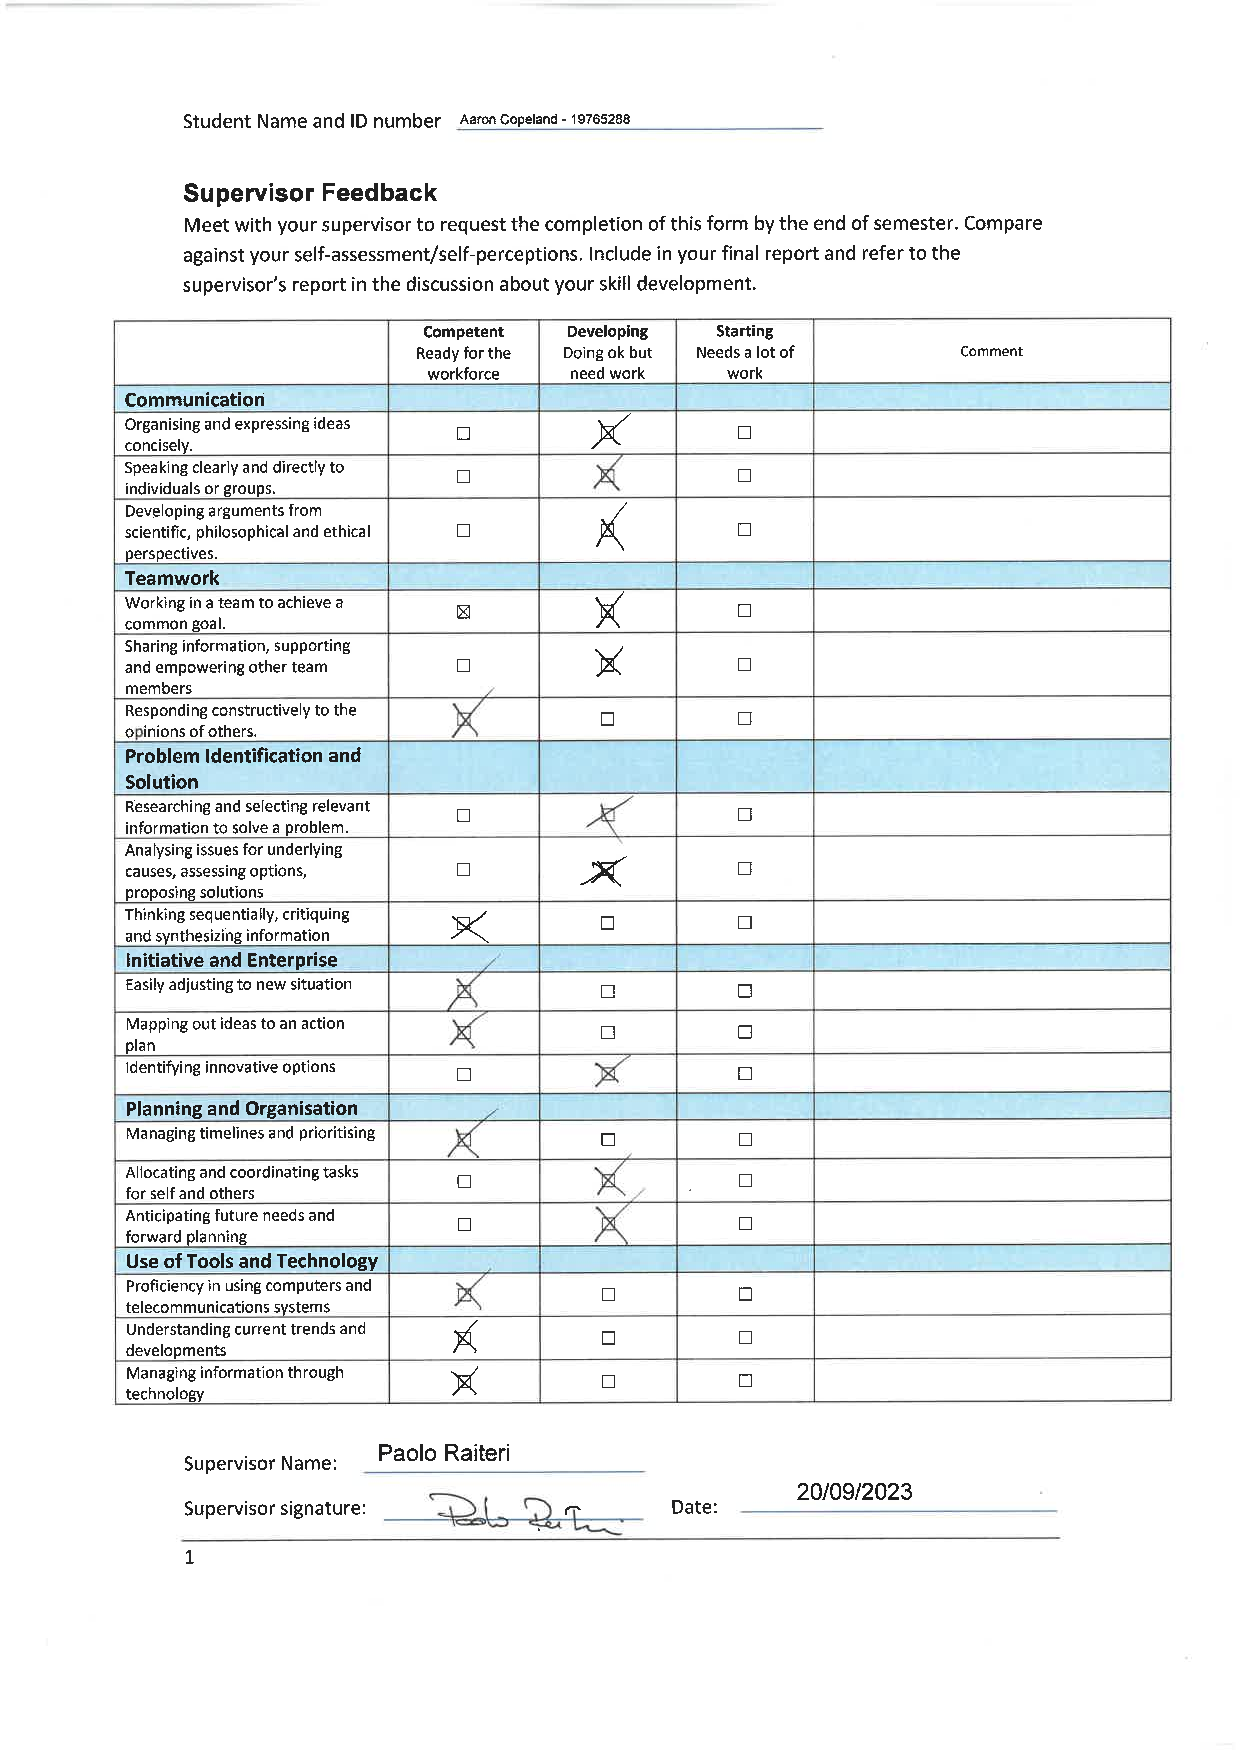
\includepdf[pages=-]{suprep.pdf}

\end{document}